\section{Experimental Studies}
\label{sec:experiment}
We examine the difference in the operation of NSGAII and SNOGA and evaluate their performance in comparison with three existing methods (ASTRAL, MP-EST and STELAR). ASTRAL and MP-EST are two of the most widely used and accurate summary methods~\cite{islam2019stelar}. We used three simulated datasets: 10-taxon (\#estimated gene tree: 200)~\cite{bayzid2015weighted}, 11-taxon (\#estimated gene tree: 50)~\cite{chung2011comparing} and 15-taxon (\#estimated gene tree: 100)~\cite{statistical-binning}. Each of them has 10 replicates (R1 to R10). We used False Negative (FN) rate~\cite{bayzid2013naive} to measure the accuracy of the estimated species tree. FN rate expresses the fraction of edges present in the true species tree (Provided with the dataset) but missing in the estimated tree. Thus the calculated FN rate of the solutions finally returned by an algorithm reflects the actual performance of that algorithm concerning the application (i.e., species tree estimation).%previously studied

For NSGAII and SNOGA, we carried out 15 independent runs due to their stochastic nature. We collected the trees estimated by ASTRAL, STELAR and MP-EST from~\cite{islam2019stelar}. They ran the exact version of ASTRAL and STELAR, which are guaranteed to return the globally optimal tree. And for MP-EST, they ran with 10 random starting points and selected the species tree with the best PL value.   

\begin{figure}[!h]
	\begin{adjustwidth}{-4cm}{-3cm}
		\centering    
		\includegraphics[width=1.6\textwidth]{Figure/tool_ratio}
	\end{adjustwidth}
	\caption{The issue of overshooting the optimization criterion beyond the true tree by existing methods. Each row shows the ratio of scores (QT/PL/TP), optimized by a particular method (ASTRAL/MP-EST/STELAR), of the true tree to that of the estimated tree by the same method.} \label{fig:tool_ratio}
	
\end{figure}

\subsection{Overshooting of Optimization Criterion}
\label{subsec:observation}
At first, we present an important observation that essentially motivated us to tackle the problem of species tree estimation as a MOP. As we mentioned in Section~\ref{sec:intro}, existing methods may overshoot the criterion they try to optimize, and thus may deviate from the true tree. In Fig.~\ref{fig:tool_ratio}, we summarize our observations for three methods (ASTRAL, MP-EST and STELAR) on 10 replicates of our selected datasets. Here, the top row shows the ratio of quartet-scores (QT) of the true trees to quartet-scores (QT) of the ASTRAL-estimated trees. Likewise, the middle row shows the pseudo-likelihood (PL) ratio of the true trees and MP-EST estimated trees and the bottom row does the same with the triplet (TP) ratio of STELAR. As we treat each objective as a minimization task, ideally these ratios should be 1 (marked as a gray horizontal line in each plot). However, we find that in most of the cases the ratio is greater than 1 implying that the results have been over-optimized. %And for 15-taxon (third column of Fig.~\ref{fig:tool_ratio}), we 


\subsection{NSGAII vs. SNOGA}
Now we closely inspect the behavioral difference between NSGAII and SNOGA to find out how SNOGA addresses the two issues (mentioned in Section~\ref{sec:problem}) in comparison with NSGAII. To ensure a level playing ground, we executed both algorithms with the same configuration (independent run: 15, population size: 100, maximum generations: 99, crossover rate: 0.3, mutation rate: 1.0). For SNOGA, we use tournament size 10.

\begin{figure}[!htbp]
	%\scriptsize
	\centering
	\begin{adjustwidth}{-1cm}{-1cm}
		\begin{subfigure}[b]{0.4\textwidth}
			\includegraphics[width=\textwidth]{Figure/10-taxon_NSGAII_corr_plot}
			\caption{NSGAII: 10-taxon}
			%\label{fig:con_pr06}
		\end{subfigure}%
		\begin{subfigure}[b]{0.4\textwidth}
			\includegraphics[width=\textwidth]{Figure/11-taxon_NSGAII_corr_plot}
			\caption{NSGAII: 11-taxon}
			%\label{fig:con_pr07}
		\end{subfigure}%
		\begin{subfigure}[b]{0.4\textwidth}
			\includegraphics[width=\textwidth]{Figure/15-taxon_NSGAII_corr_plot}
			\caption{NSGAII: 15-taxon}
			%\label{fig:con_pr09}
		\end{subfigure}    
		\begin{subfigure}[b]{0.4\textwidth}
			\includegraphics[width=\textwidth]{Figure/10-taxon_NOSSGA_corr_plot}
			\caption{SNOGA: 10-taxon}
			%\label{fig:con_pr06}
		\end{subfigure}%
		\begin{subfigure}[b]{0.4\textwidth}
			\includegraphics[width=\textwidth]{Figure/11-taxon_NOSSGA_corr_plot}
			\caption{SNOGA: 11-taxon}
			%\label{fig:con_pr07}
		\end{subfigure}%
		\begin{subfigure}[b]{0.4\textwidth}
			\includegraphics[width=\textwidth]{Figure/15-taxon_NOSSGA_corr_plot}
			\caption{SNOGA: 15-taxon}
			%\label{fig:con_pr09}
		\end{subfigure}
		\caption{Correlations between each pair of objectives against generations for NSGAII and SNOGA on three datasets.}
		\label{fig:gen_wise_correlation}
	\end{adjustwidth}
\end{figure}

\subsubsection{Correlation between two objectives:} We plot the correlation coefficients between each pair of objectives against different generations for NSGAII and SNOGA on three datasets in Fig.~\ref{fig:gen_wise_correlation}. Here the horizontal axis represents the generations and the vertical axis represents the correlation coefficients averaged over 15 runs and 10 replicates. We see that, contrary to NSGAII, SNOGA does not exhibit any negative correlation coefficient between any pair of objectives. These results suggest that SNOGA is able to prevent the optimization of one objective to a great extent even at the loss of some other objectives, thereby alleviating issue~\ref{item:i1} (mentioned in Section~\ref{sec:problem}) to some extent.% as an attempt to resolve  (please see Section~\ref{sec:problem}) as we discussed earlier in Section~\ref{sec:method}). %objective to a great extent according to our requirement\footnote{Nayeem link it to the method section in algo}. 

\begin{figure}[!htbp]
	\centering
	\begin{adjustwidth}{-1cm}{-1cm}
		\begin{subfigure}[b]{0.4\textwidth}
			\includegraphics[width=\textwidth]{Figure/10-taxon_NSGAII_std_dev}
			\caption{NSGAII: 10-taxon}
			%\label{fig:con_pr06}
		\end{subfigure}%
		\begin{subfigure}[b]{0.4\textwidth}
			\includegraphics[width=\textwidth]{Figure/11-taxon_NSGAII_std_dev}
			\caption{NSGAII: 11-taxon}
			%\label{fig:con_pr07}
		\end{subfigure}%
		\begin{subfigure}[b]{0.4\textwidth}
			\includegraphics[width=\textwidth]{Figure/15-taxon_NSGAII_std_dev}
			\caption{NSGAII: 15-taxon}
			%\label{fig:con_pr09}
		\end{subfigure}
		\begin{subfigure}[b]{0.4\textwidth}
			\includegraphics[width=\textwidth]{Figure/10-taxon_NOSSGA_std_dev}
			\caption{SNOGA: 10-taxon}
			%\label{fig:con_pr06}
		\end{subfigure}%
		\begin{subfigure}[b]{0.4\textwidth}
			\includegraphics[width=\textwidth]{Figure/11-taxon_NOSSGA_std_dev}
			\caption{SNOGA: 11-taxon}
			%\label{fig:con_pr07}
		\end{subfigure}%
		\begin{subfigure}[b]{0.4\textwidth}
			\includegraphics[width=\textwidth]{Figure/15-taxon_NOSSGA_std_dev}
			\caption{SNOGA: 15-taxon}
			%\label{fig:con_pr09}
		\end{subfigure}
		\caption{Variation of standard deviation of three objectives and FN rates in the population with generations for NSGAII and SNOGA on three datasets.
			% on three datasets. The plotted standard deviations are averaged over 15 runs and 10 replicates. 
		}
		\label{fig:gen_wise_std_dev}
	\end{adjustwidth}
\end{figure}

\subsubsection{Diversity of objectives and FN rate:}\label{subsubsec:diversity} Fig.~\ref{fig:gen_wise_std_dev} shows the variation of the standard deviation of three objective values (normalized using global maximum and minimum) of the population members and their respective FN rates in the population with generations for NSGAII and SNOGA on three datasets. Along the vertical axis, we plotted the standard deviation values averaged over 15 runs and 10 replicates. We find that SNOGA can maintain diversity throughout the generations presumably owing to the steps taken to mitigate issue~\ref{item:i2} which we discussed in Section~\ref{sec:method}. On the other hand, NSGAII loses diversity at an early stage.
%These figures clearly show that NSGAII loses diversity at an early stage possibly. This an outcome of not taking necessary measures to tackle issue~\ref{item:i2}~\cite{qu2010multi}. \footnote{The knowledge of FN rate is absent to the EMOs.}   

\begin{figure}[!h]
	\centering
	\begin{adjustwidth}{-1cm}{-1cm}
		\begin{subfigure}[b]{0.4\textwidth}
			\includegraphics[width=\textwidth]{Figure/10-taxon_NSGAII_minimum}
			\caption{NSGAII: 10-taxon}
			%\label{fig:con_pr06}
		\end{subfigure}%
		\begin{subfigure}[b]{0.4\textwidth}
			\includegraphics[width=\textwidth]{Figure/11-taxon_NSGAII_minimum}
			\caption{NSGAII: 11-taxon}
			%\label{fig:con_pr07}
		\end{subfigure}%
		\begin{subfigure}[b]{0.4\textwidth}
			\includegraphics[width=\textwidth]{Figure/15-taxon_NSGAII_minimum}
			\caption{NSGAII: 15-taxon}
			%\label{fig:con_pr09}
		\end{subfigure}
		\begin{subfigure}[b]{0.4\textwidth}
			\includegraphics[width=\textwidth]{Figure/10-taxon_NOSSGA_minimum}
			\caption{SNOGA: 10-taxon}
			%\label{fig:con_pr06}
		\end{subfigure}%
		\begin{subfigure}[b]{0.4\textwidth}
			\includegraphics[width=\textwidth]{Figure/11-taxon_NOSSGA_minimum}
			\caption{SNOGA: 11-taxon}
			%\label{fig:con_pr07}
		\end{subfigure}%
		\begin{subfigure}[b]{0.4\textwidth}
			\includegraphics[width=\textwidth]{Figure/15-taxon_NOSSGA_minimum}
			\caption{SNOGA: 15-taxon}
			%\label{fig:con_pr09}
		\end{subfigure}
		\caption{Variation of minimum of three objectives (individually) and FN rates in the population with generations for NSGAII and SNOGA on three datasets.
			%The plotted minimum values are averaged over 15 runs and 10 replicates. 
		}
		\label{fig:gen_wise_min}
	\end{adjustwidth}
\end{figure}

\subsubsection{Improvement of FN rate vs. individual objectives:} Now we observe how the best (minimum) value of three objectives (individually) and FN rate (lower is better) in the population behave across generations for NSGAII and SNOGA as depicted in Fig.~\ref{fig:gen_wise_min}. The plotted values are averaged over 15 runs and 10 replicates. We mentioned earlier that FN rate reflects the true performance of an algorithm. However, the FN rate is not the fitness criterion of the optimization process. Rather, the optimization continues based on the three objective values (QT, TP and PL).
%But its knowledge is absent to the algorithm.
We see that, NSGAII allows one or more objectives to improve as much as possible which may cause the resultant species tree to deviate from the true tree (issue~\ref{item:i1}). As a result, the best FN rate of NSGAII starts to degrade after a particular generation despite continuous improvement of some objectives. For example, in Fig.~\ref{fig:gen_wise_min}(a), NSGAII achieves the best FN rate at around $ 30^{th} $ generation. Afterwards, the FN rate starts to degrade. However, QT and TP continue to improve until $ 50^{th} $ and $ 80^{th} $ generation respectively.
On the other hand, to avoid such deviation, SNOGA in effect, restricts the improvement of one or more objectives after certain number of generation. So its FN rate continues to improve. From these results, we can see that SNOGA is more effective than NSGAII in dealing issue~\ref{item:i1}.%(except PL\footnote{To decrease the large runtime of PL calculation using MP-EST, we decreased the default iteration count})


\subsubsection{Comparison based on hypervolume:} We mentioned in Section~\ref{sec:problem} that the problem that we deal with in this paper is different from the traditional MOPs. Importantly, the definition of convergence for MOPs is not the same as the convergence within the context of this problem. To explore this issue, we compare NSGAII and SNOGA in terms of hypervolume (HV)~\cite{zitzler1999multiobjective} which is probably the most popular performance measure used for MOPs. HV captures both convergence and diversity of the PF, sampled by an EMO algorithm, in a single real-value. For MOPs with all minimization objectives, a higher value of HV is desirable. In Fig.~\ref{fig:gen_wise_hv}, we plot the HV values for NSGAII and SNOGA which are averaged over 15 runs and 10 replicates. From these results, it is difficult to differentiate between these two algorithms. Both HV values get saturated at an early generation. Even, according to HV, SNOGA seems better than NSGAII more strikingly so for the larger dataset. The reason for worse value of NSGAII concerning HV could be attributed to the loss of diversity, as exhibited by it, at an early stage. 

\begin{figure}[!htbp]
	\centering
	\begin{adjustwidth}{-1cm}{-1cm}
		\begin{subfigure}[b]{0.4\textwidth}
			\includegraphics[width=\textwidth]{Figure/10-taxon_hv}
			\caption{10-taxon}
			%\label{fig:con_pr06}
		\end{subfigure}%
		\begin{subfigure}[b]{0.4\textwidth}
			\includegraphics[width=\textwidth]{Figure/11-taxon_hv}
			\caption{11-taxon}
			%\label{fig:con_pr07}
		\end{subfigure}%
		\begin{subfigure}[b]{0.4\textwidth}
			\includegraphics[width=\textwidth]{Figure/15-taxon_hv}
			\caption{15-taxon}
			%\label{fig:con_pr09}
		\end{subfigure}
		\caption{Variation of HV with generations for NSGAII and SNOGA on three datasets.}
		\label{fig:gen_wise_hv}
	\end{adjustwidth}
\end{figure}

\begin{figure}
	\centering
	\begin{adjustwidth}{-4cm}{-2cm}
		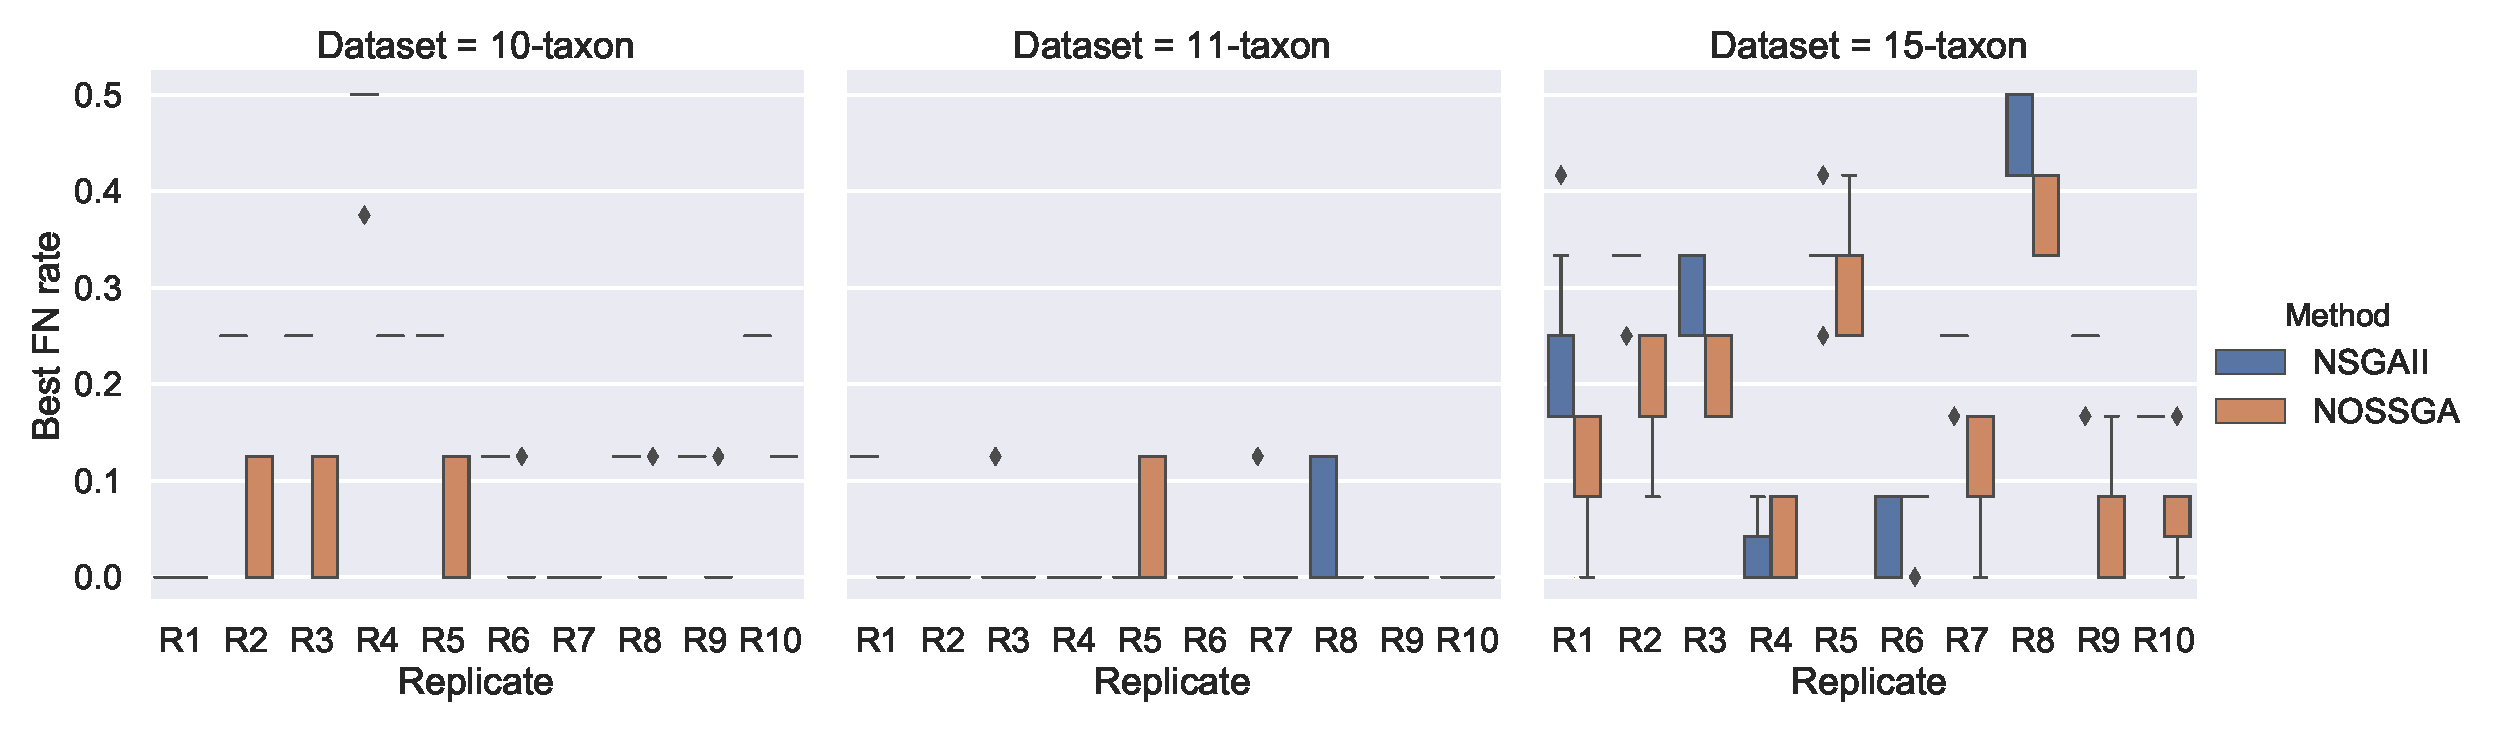
\includegraphics[width=1.7\textwidth]{Figure/emo_boxplot}
	\end{adjustwidth}
	\caption{Accuracy of the best estimated species trees extracted from the final population of NSGAII and SNOGA on each dataset having 10 replicate.} \label{fig:emo_compare}
	
\end{figure}

\subsubsection{Comparison based on Tree accuracy:} Finally we compare NSGAII and SNOGA in terms of the tree accuracy for 10 replicates of each dataset. We measure the tree accuracy in terms of FN rate. A lower value of FN rate corresponds to a higher accuracy. We graphically summarize the FN rate of the best trees obtained from the final population of 15 independent runs using boxplots in Fig.~\ref{fig:emo_compare}. We observe that SNOGA can offer much better solutions than NSGAII in most of the cases. In some situations, two algorithms perform equally.

\begin{figure}
	\begin{adjustwidth}{0cm}{0cm}
		\centering
		\includegraphics[width=1.0\textwidth]{Figure/all_dataset_compare}
		\caption{Performance comparison of ASTRAL, STELAR, MP-EST, NSGAII and SNOGA on three datasets. 
			%We show the average FN rates with standard error bars over 10 replicates
		} \label{fig:compare_exisitng_methods}
	\end{adjustwidth}
\end{figure}

\subsection{Comparison with Existing Methods}
We evaluated the best trees offered by NSGAII and SNOGA in comparison with the output of ASTRAL, MP-EST and STELAR. On each dataset, we ran both NSGAII and SNOGA only for 99 generations (population size: 100, function evaluations: 10000). 
Fig.~\ref{fig:compare_exisitng_methods} shows the average FN rates with standard error bars over 10 replicates. We find that SNOGA offers the highest accuracy among all. On the 10-taxon dataset, SNOGA can achieve nearly 4X accuracy than ASTRAL. For the rest two datasets, the accuracy improvement is around 2X compared to ASTRAL. Interestingly, even the basic NSGAII exhibits more accuracy than the three existing methods. So the advantage of formulating this problem as a MOP is obvious. From actual application point of view, if we run the original NSGAII algorithm for a large number of generations its accuracy may fall for not resolving the issues mentioned in Section~\ref{sec:problem} properly which we saw earlier. Note that the FN rate is not the fitness criterion of the optimization process. Rather, the optimization continues based on the objective values.
So we can state that, owing to the characteristics designed considering the problem nature, SNOGA achieves at least 1.4X accuracy gain over the original NSGAII in all datasets. 



%\subsection{Discussion}

\begin{comment}
\begin{figure}[!htbp]
\centering
\begin{adjustwidth}{-1cm}{}
\begin{subfigure}[b]{0.55\textwidth}
\includegraphics[width=\textwidth]{Figure/10-taxon_10_replicates}
\caption{10-taxon}
%\label{fig:con_pr06}
\end{subfigure}%
\begin{subfigure}[b]{0.55\textwidth}
\includegraphics[width=\textwidth]{Figure/11-taxon_10_replicates}
\caption{11-taxon}
%\label{fig:con_pr07}
\end{subfigure}%
%    \newline

\begin{subfigure}[b]{0.55\textwidth}
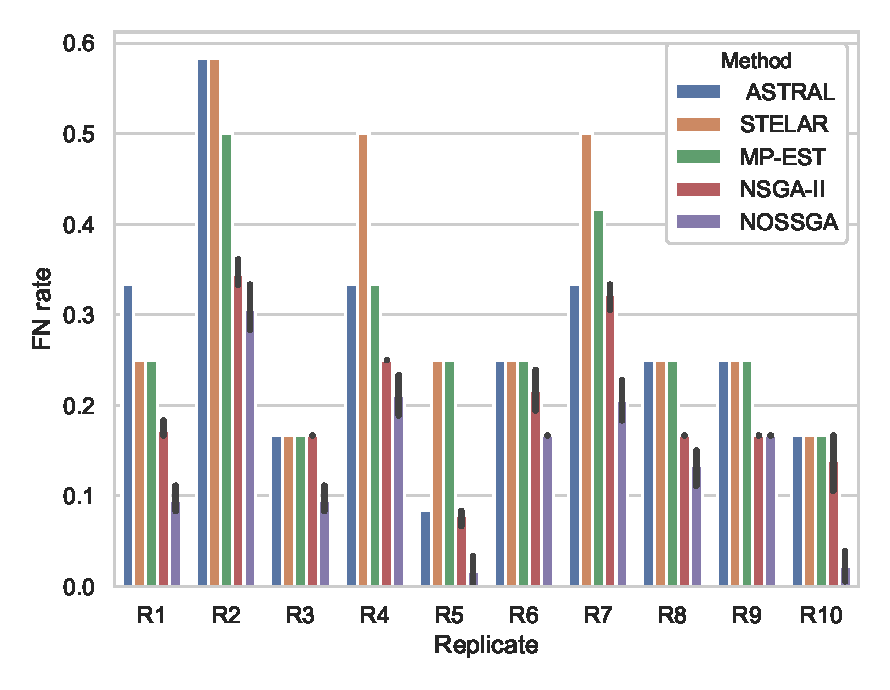
\includegraphics[width=\textwidth]{Figure/15-taxon_10_replicates}
\caption{15-taxon}
%\label{fig:con_pr09}
\end{subfigure}
\begin{subfigure}[b]{0.55\textwidth}
\includegraphics[width=\textwidth]{Figure/all_dataset_compare}
\caption{Summary}
%\label{fig:con_pr09}
\end{subfigure}%

\caption{Comparison of ASTRAL, STELAR, MP-EST, NSGAII and SNOGA on 10 replicates of 3 datasets.}
\label{fig:datasets}
\end{adjustwidth}
\end{figure}



\begin{figure}[!htbp]
\centering
\begin{adjustwidth}{-1cm}{}
\begin{subfigure}[b]{0.48\textwidth}
\includegraphics[width=\textwidth]{Figure/10-taxon_NSGA-II_heatmap}
\caption{NSGAII: 10-taxon}
%\label{fig:con_pr06}
\end{subfigure}%
\begin{subfigure}[b]{0.4\textwidth}
\includegraphics[width=\textwidth]{Figure/11-taxon_NSGA-II_heatmap}
\caption{NSGAII: 11-taxon}
%\label{fig:con_pr07}
\end{subfigure}%
\begin{subfigure}[b]{0.4\textwidth}
\includegraphics[width=\textwidth]{Figure/15-taxon_NSGA-II_heatmap}
\caption{NSGAII: 15-taxon}
%\label{fig:con_pr09}
\end{subfigure}

\begin{subfigure}[b]{0.48\textwidth}
\includegraphics[width=\textwidth]{Figure/10-taxon_NOSSGA_heatmap}
\caption{SNOGA: 10-taxon}
%\label{fig:con_pr06}
\end{subfigure}%
\begin{subfigure}[b]{0.4\textwidth}
\includegraphics[width=\textwidth]{Figure/11-taxon_NOSSGA_heatmap}
\caption{SNOGA: 11-taxon}
%\label{fig:con_pr07}
\end{subfigure}%
\begin{subfigure}[b]{0.4\textwidth}
\includegraphics[width=\textwidth]{Figure/15-taxon_NOSSGA_heatmap}
\caption{SNOGA: 15-taxon}
%\label{fig:con_pr09}
\end{subfigure}
\caption{Correlation between each pair of objectives as the generation of an EMO progresses. For each dataset, we average the correlation coefficient over 15 runs and 10 replicates.}
\label{fig:gen_wise_correlation}
\end{adjustwidth}
\end{figure}
%\begin{figure}
%    \centering
%    \includegraphics[width=0.6\textwidth]{Figure/10-taxon_10_replicates}
%    \caption{10-taxon.} \label{fig1}
%\end{figure}
%\begin{figure}
%    \centering
%    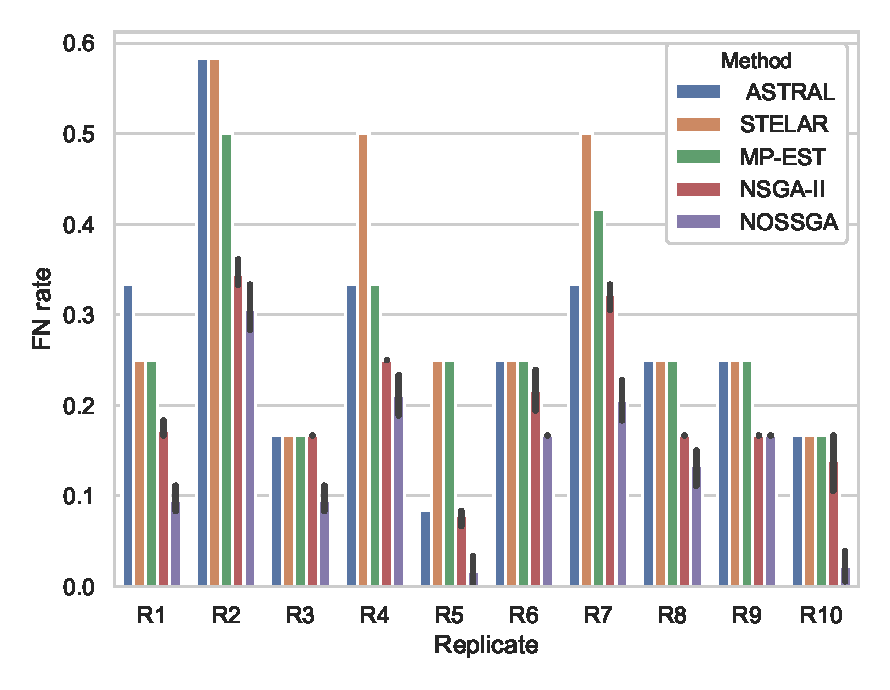
\includegraphics[width=0.6\textwidth]{Figure/15-taxon_10_replicates}
%    \caption{15-taxon.} \label{fig2}
%\end{figure}
\subsection{Results on 10-taxon dataset}
\subsection{Results on 11-taxon dataset}
\subsection{Results on 15-taxon dataset}
\end{comment}

